\documentclass[aspectratio=43,10pt]{beamer}
% supported values for aspectratio: 43, 1610, 169

\mode<presentation>
\usepackage{caption}
\usepackage{amsmath}
\usepackage{bbm}
\usepackage[utf8]{inputenc}
\usepackage[ngerman]{babel}
\usepackage{caption}
\usepackage{graphicx}
\usefonttheme{professionalfonts}
\usepackage{natbib}
\captionsetup[figure]{font=footnotesize, labelfont=small}

%%% Adjust color style in: beamerthemeTUBlayout.sty

\setbeamertemplate{navigation symbols}{}
\usetheme{TUBlayout}

%%% Adjust title image and affiliation/collaboration logos in 
% - titleimg.tikz
% - logos.tikz
%%% They are used in: beamerouterthemeTUBlayout.sty

\title[Scoring Rules]{Scoring Rules for Probabilistic Forecasting}
\author[Loay, Jonas]{Loay Hefni\inst{1}, Jonas Persé\inst{1}}
\institute[Mathematics]{\inst{1}Mathematics}
\newcommand{\preslocation}{Seminar talk on Scoring Rules for Probabilistic Forecasting}
\date{27. November 2025}

\makeindex

\begin{document}
  \frame[plain]{\titlepage}


\section{Intro}
\begin{frame}{Motivation}
    \begin{figure}
        \centering
        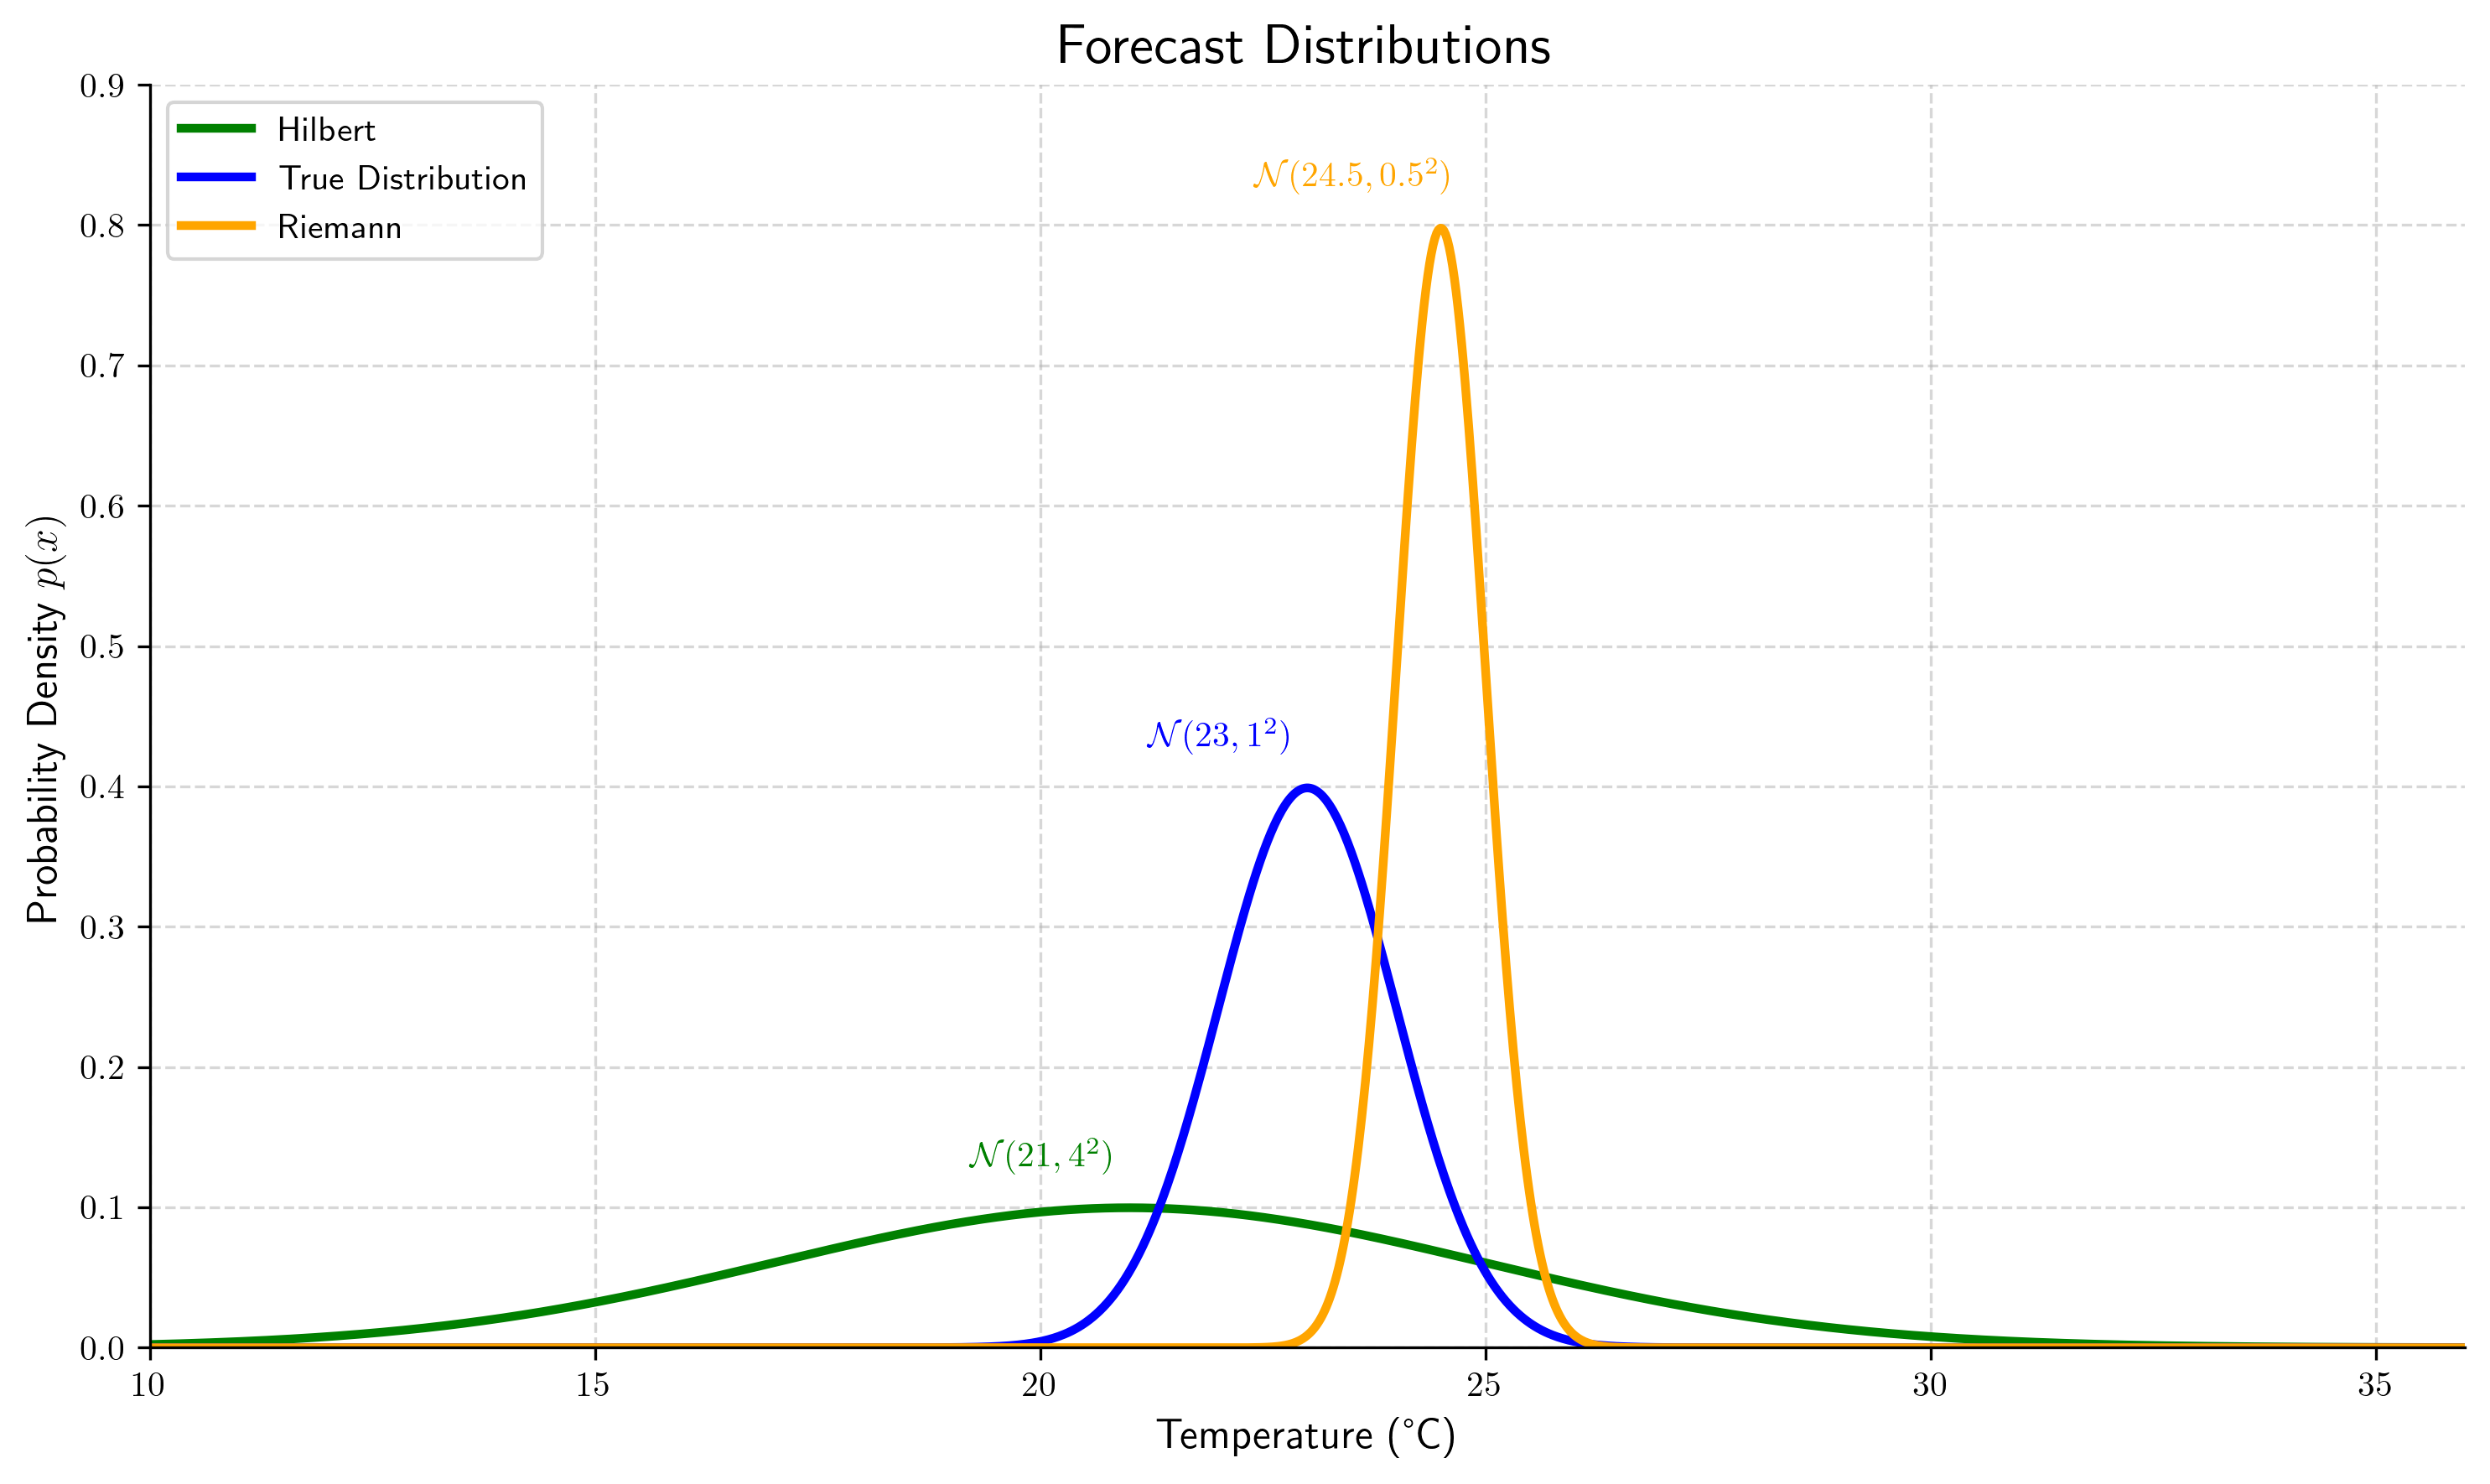
\includegraphics[width=0.8\textwidth]{images/forecast-distribution-intro0.png}\\
        $S(P, \omega) := \log(p(\omega))$
    \end{figure}
\end{frame}
\begin{frame}{Motivation}
    \begin{figure}
        \centering
        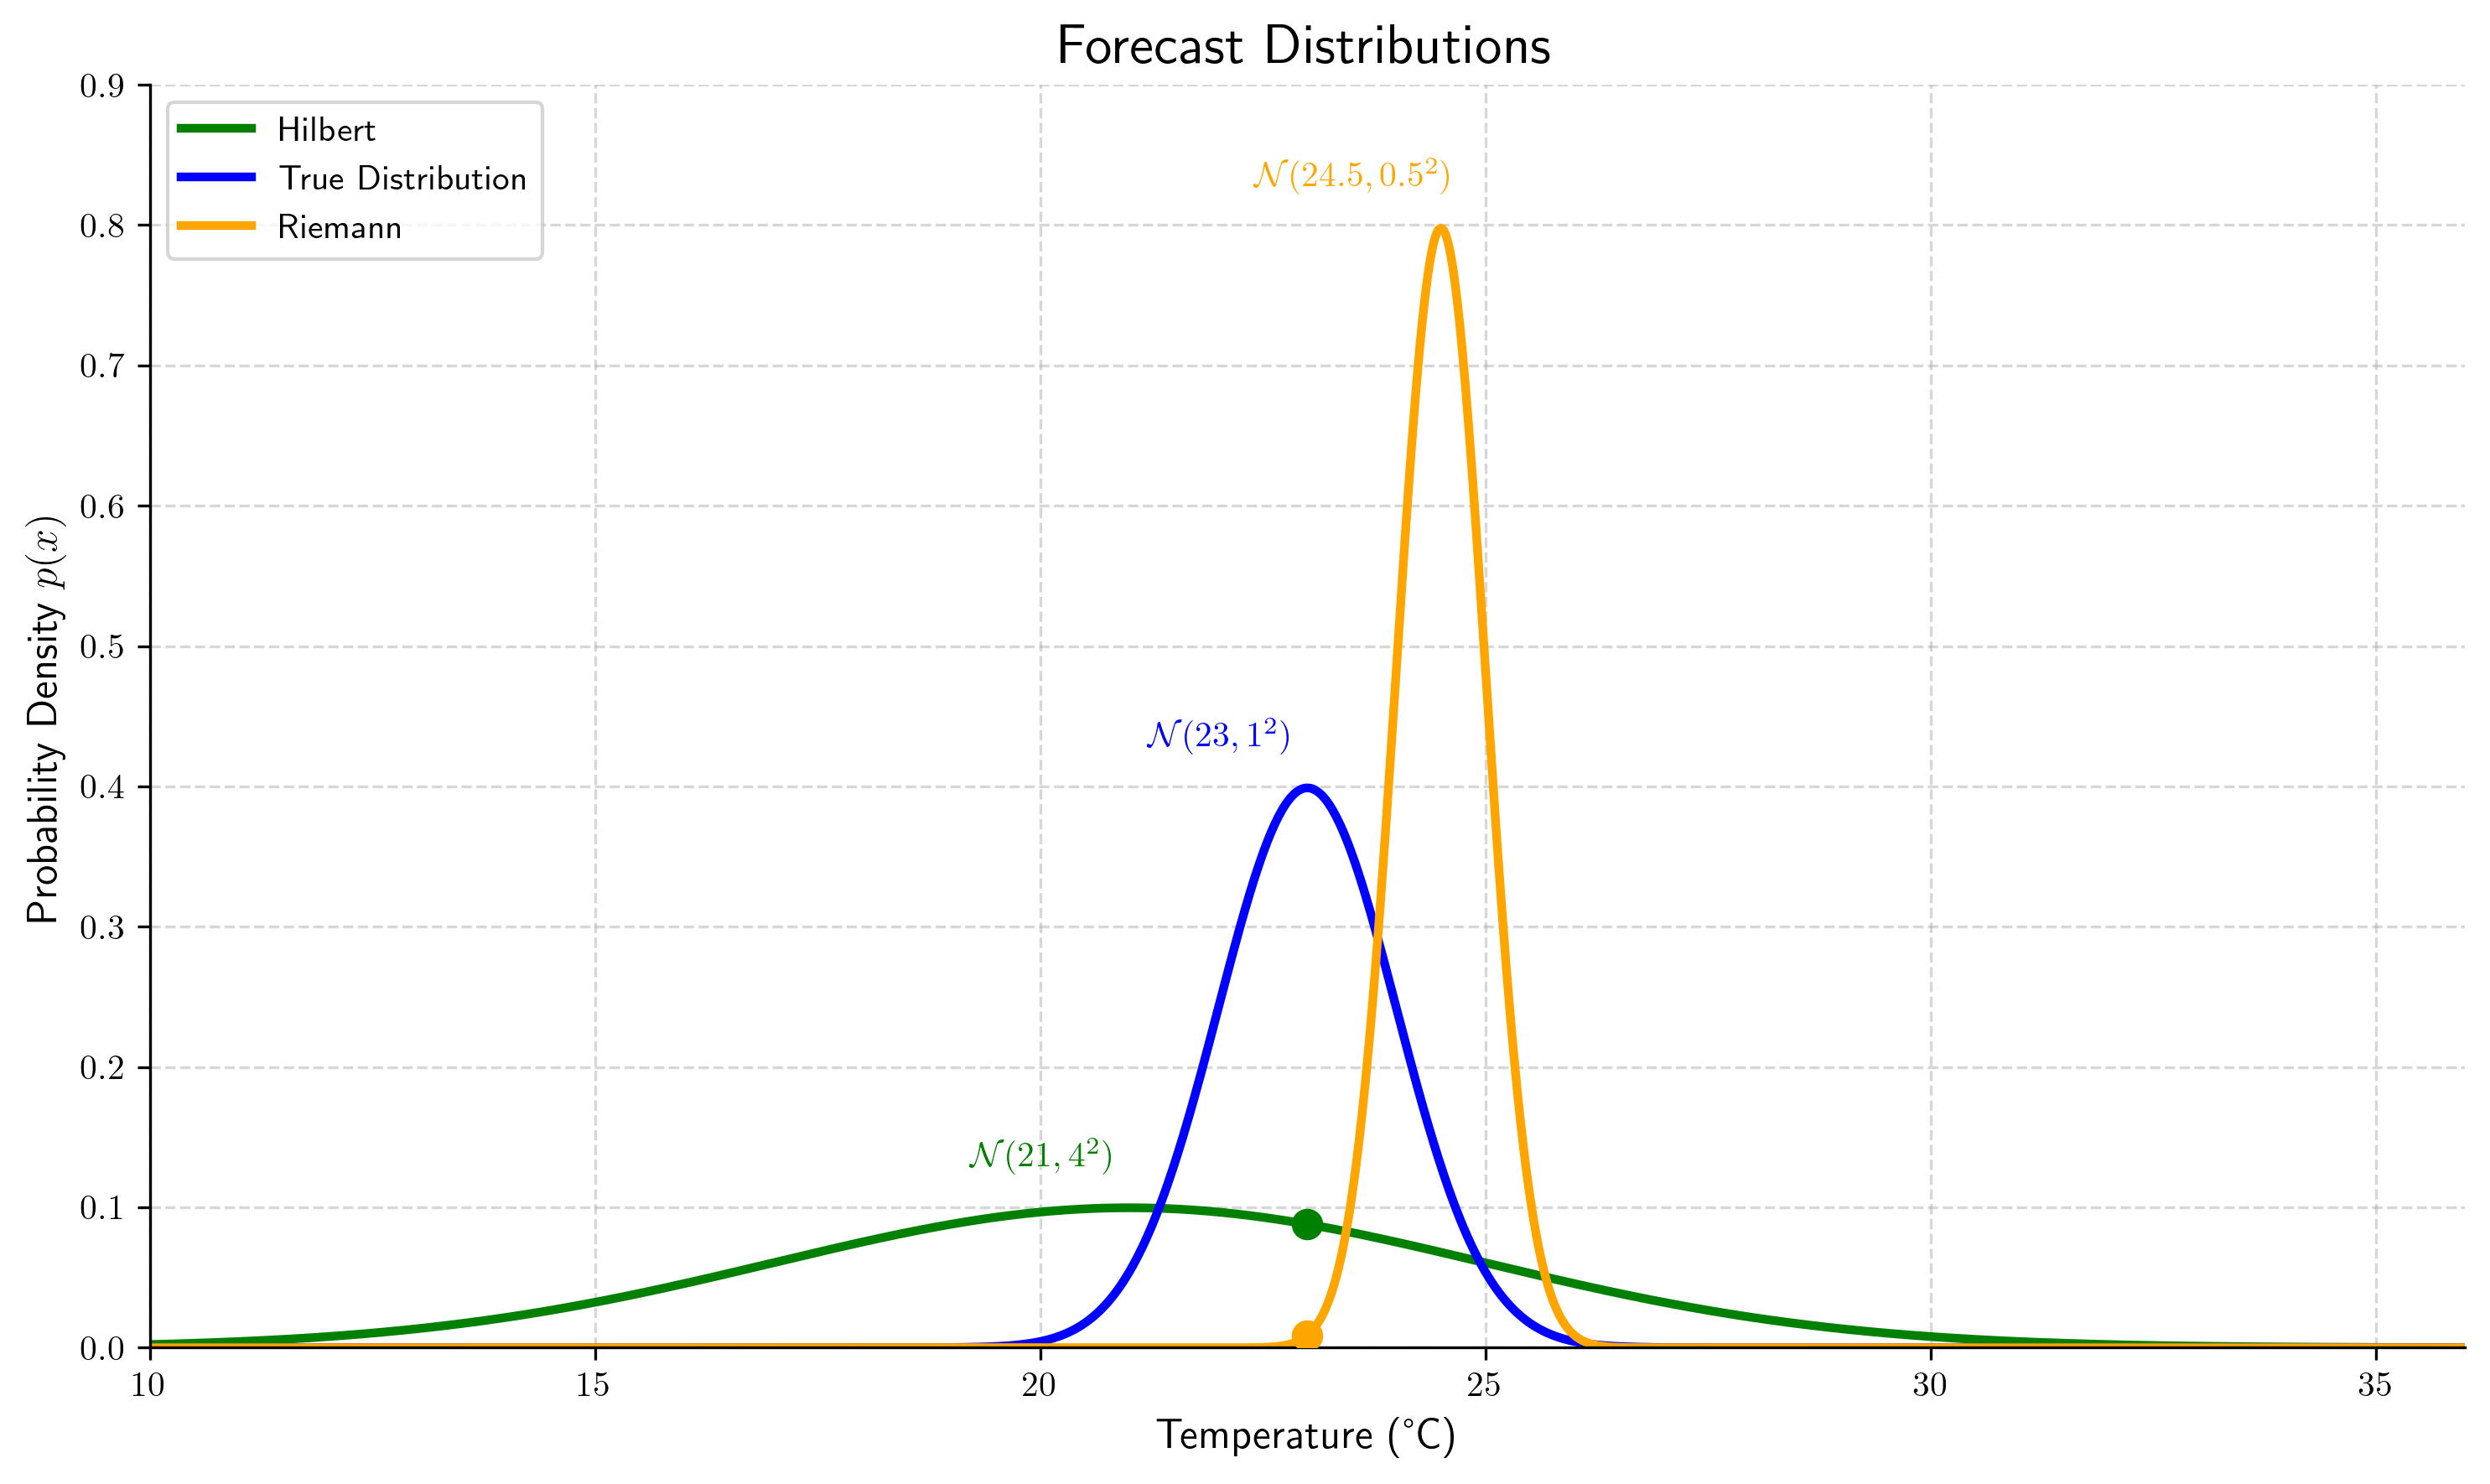
\includegraphics[width=0.8\textwidth]{images/forecast-distribution-intro1.png}\\
        Hilbert: $S(P_H, 23) = \log(p_H(23)) \approx -2.4$\\
        Riemann: $S(P_R, 23) = \log(p_R(23)) \approx -4.7$
    \end{figure}
\end{frame}
\begin{frame}{Motivation}
    \begin{figure}
        \centering
        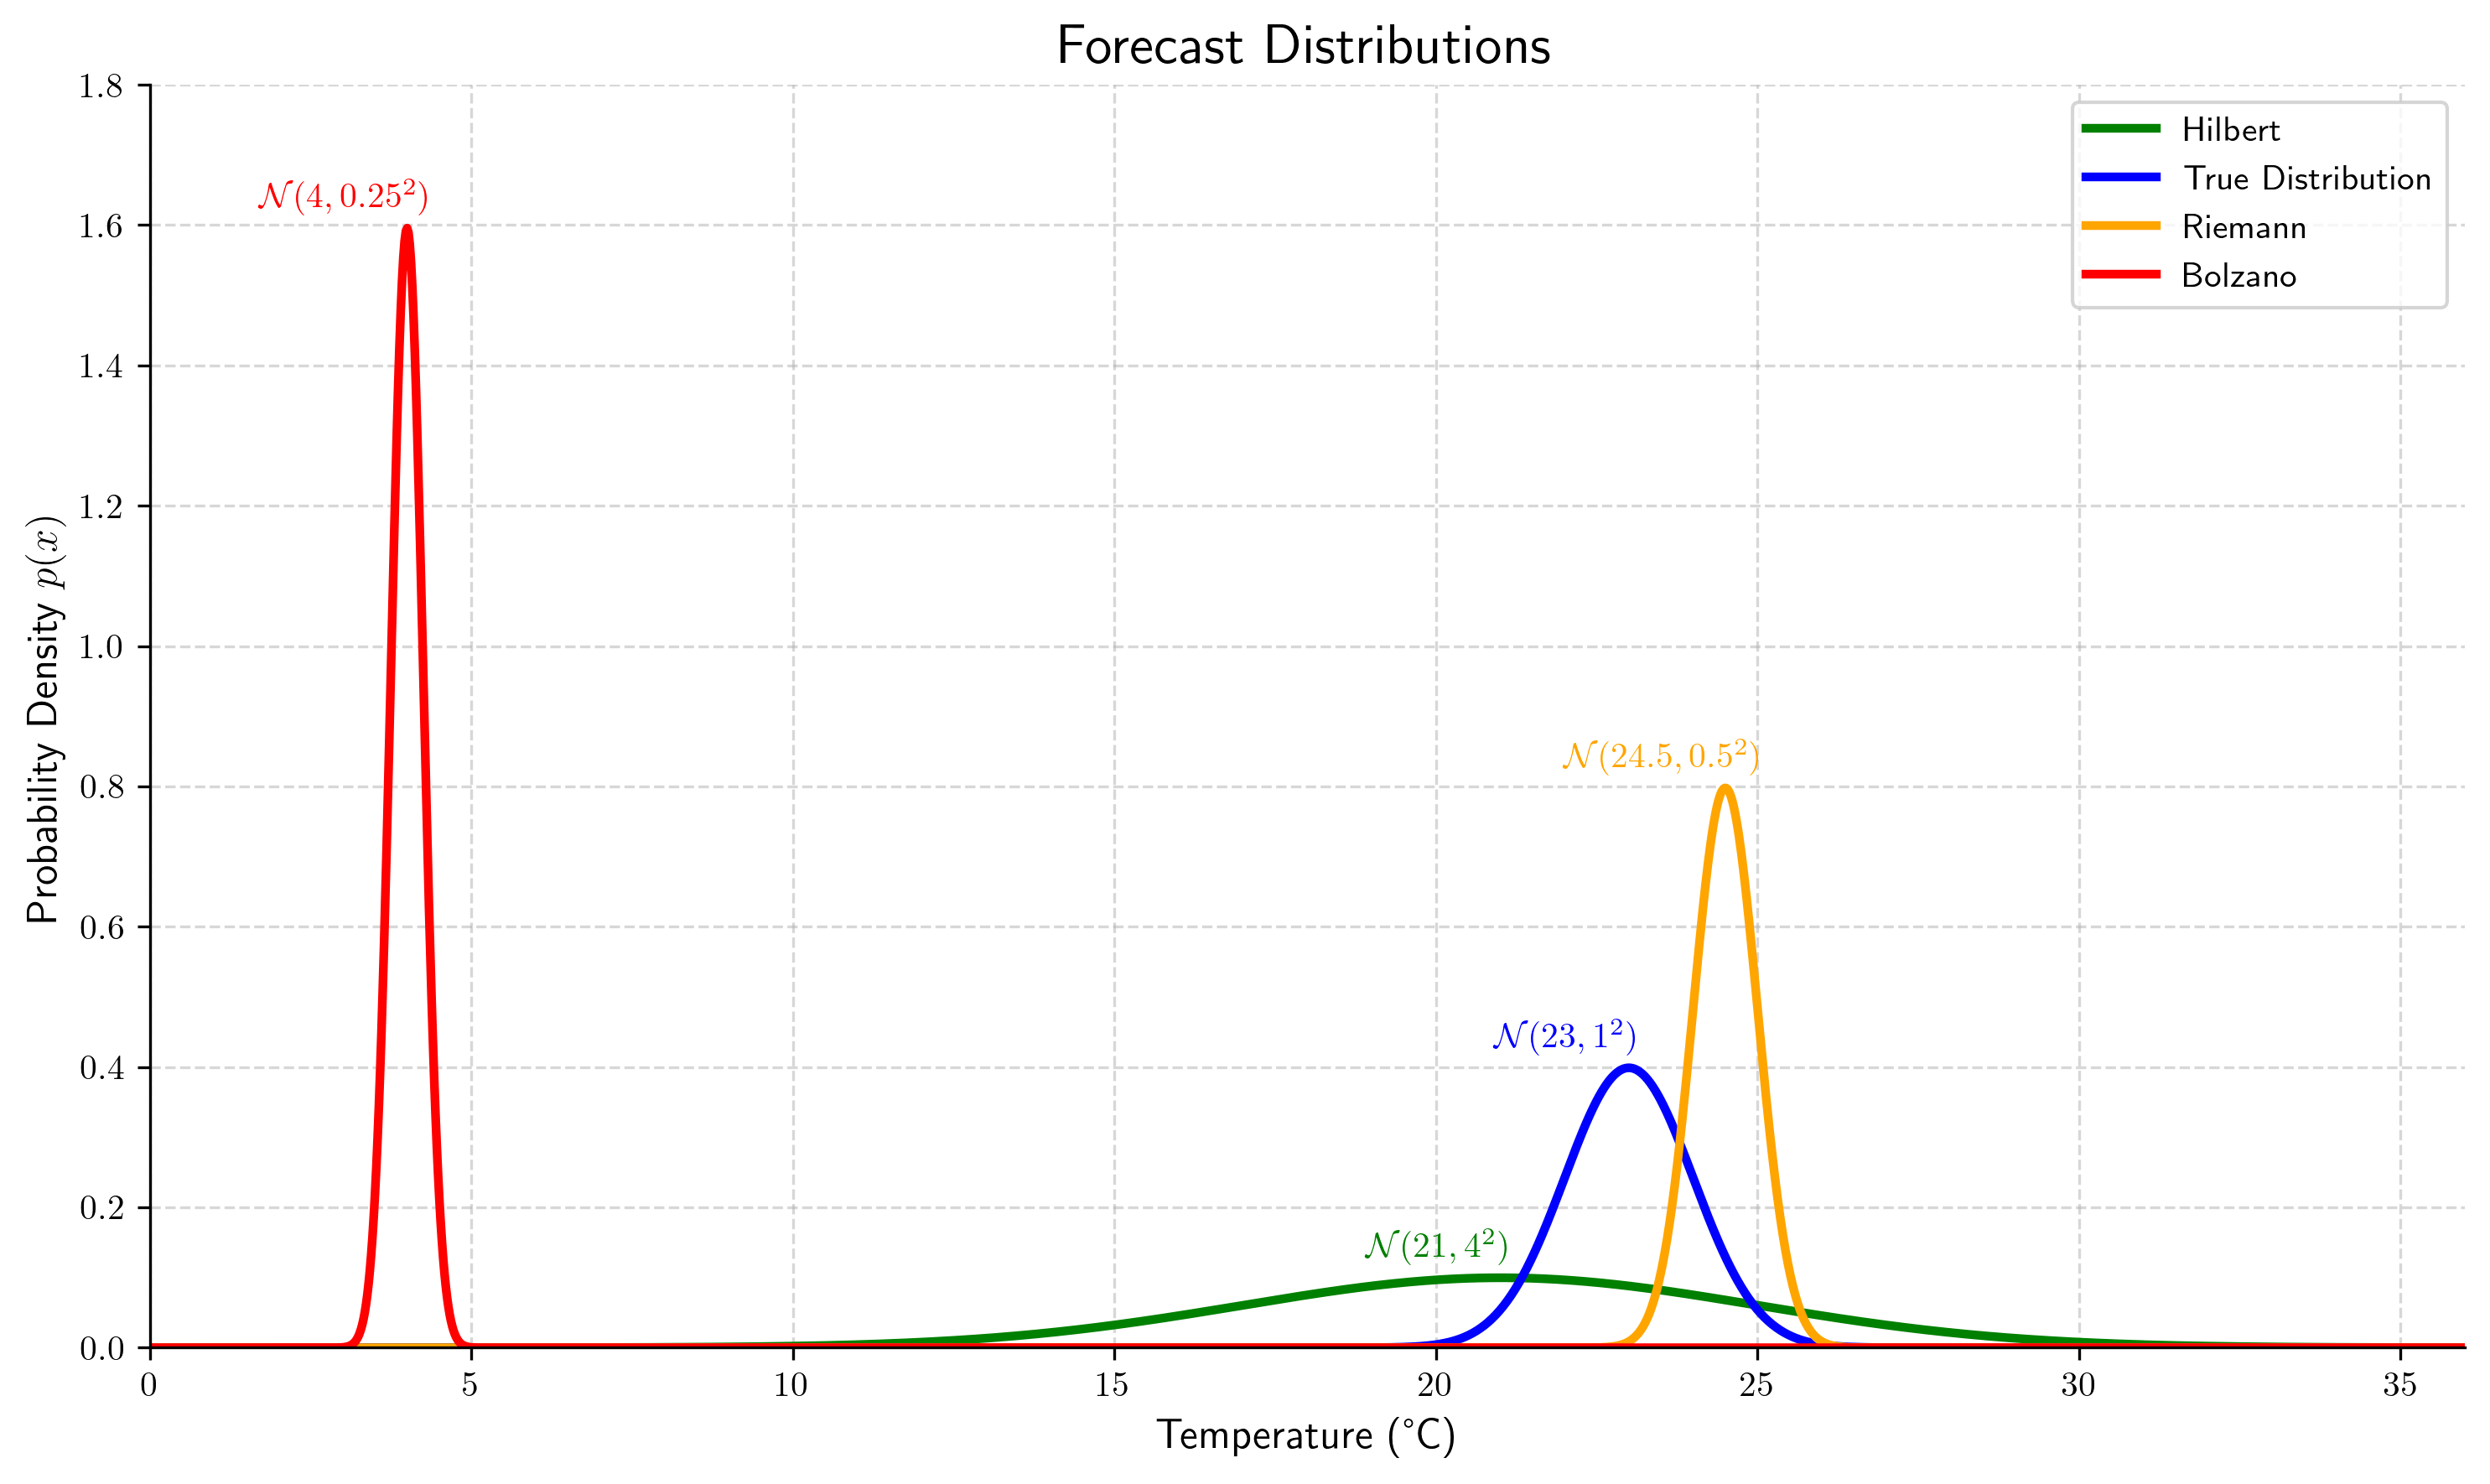
\includegraphics[width=0.8\textwidth]{images/forecast-distribution-intro2.png}\\
        Hilbert: $S(P_H, 4) = \log(p_H(4)) \approx -11.3$\\
        Riemann: $S(P_R, 4) = \log(p_R(4)) \approx -840.7$\\
        Bolzano: $S(P_B, 4) = \log(p_B(4)) \approx -0.2$
    \end{figure}
\end{frame}
\begin{frame}{Expected Score}
    \begin{block}{Definition}
        Let $Q$ be the true distribution, then
        $$S(P, Q) = \mathbb{E}^{Q}\left[ S(P, \omega)\right]$$
        is called the \textbf{Expected Score}.
    \end{block}
\end{frame}
\begin{frame}{Properness}
    Fourier knows the truth $Q$. Should he also forecast $Q$?
    \pause
    \begin{block}{Definition}
        A scoring rule is called (strictly) \textbf{proper}, if
        $$S(Q, Q) \geq S(P, Q)$$
        for all $P$.
    \end{block}
\end{frame}
\begin{frame}{Improper Scoring Rule}

    \begin{exampleblock}{Linear Score}
        Define $$S(P, \omega) := \left | \omega - \mathrm{median}(P)\right|$$
        Let $Q$ be Log-Normal. Fourier would rather predict $P\sim\mathcal{N}(23, \sigma^2)$. Then $S$ is improper $$S(P, Q) > S(Q, Q).$$
    \end{exampleblock}
    \begin{figure}
        \centering
        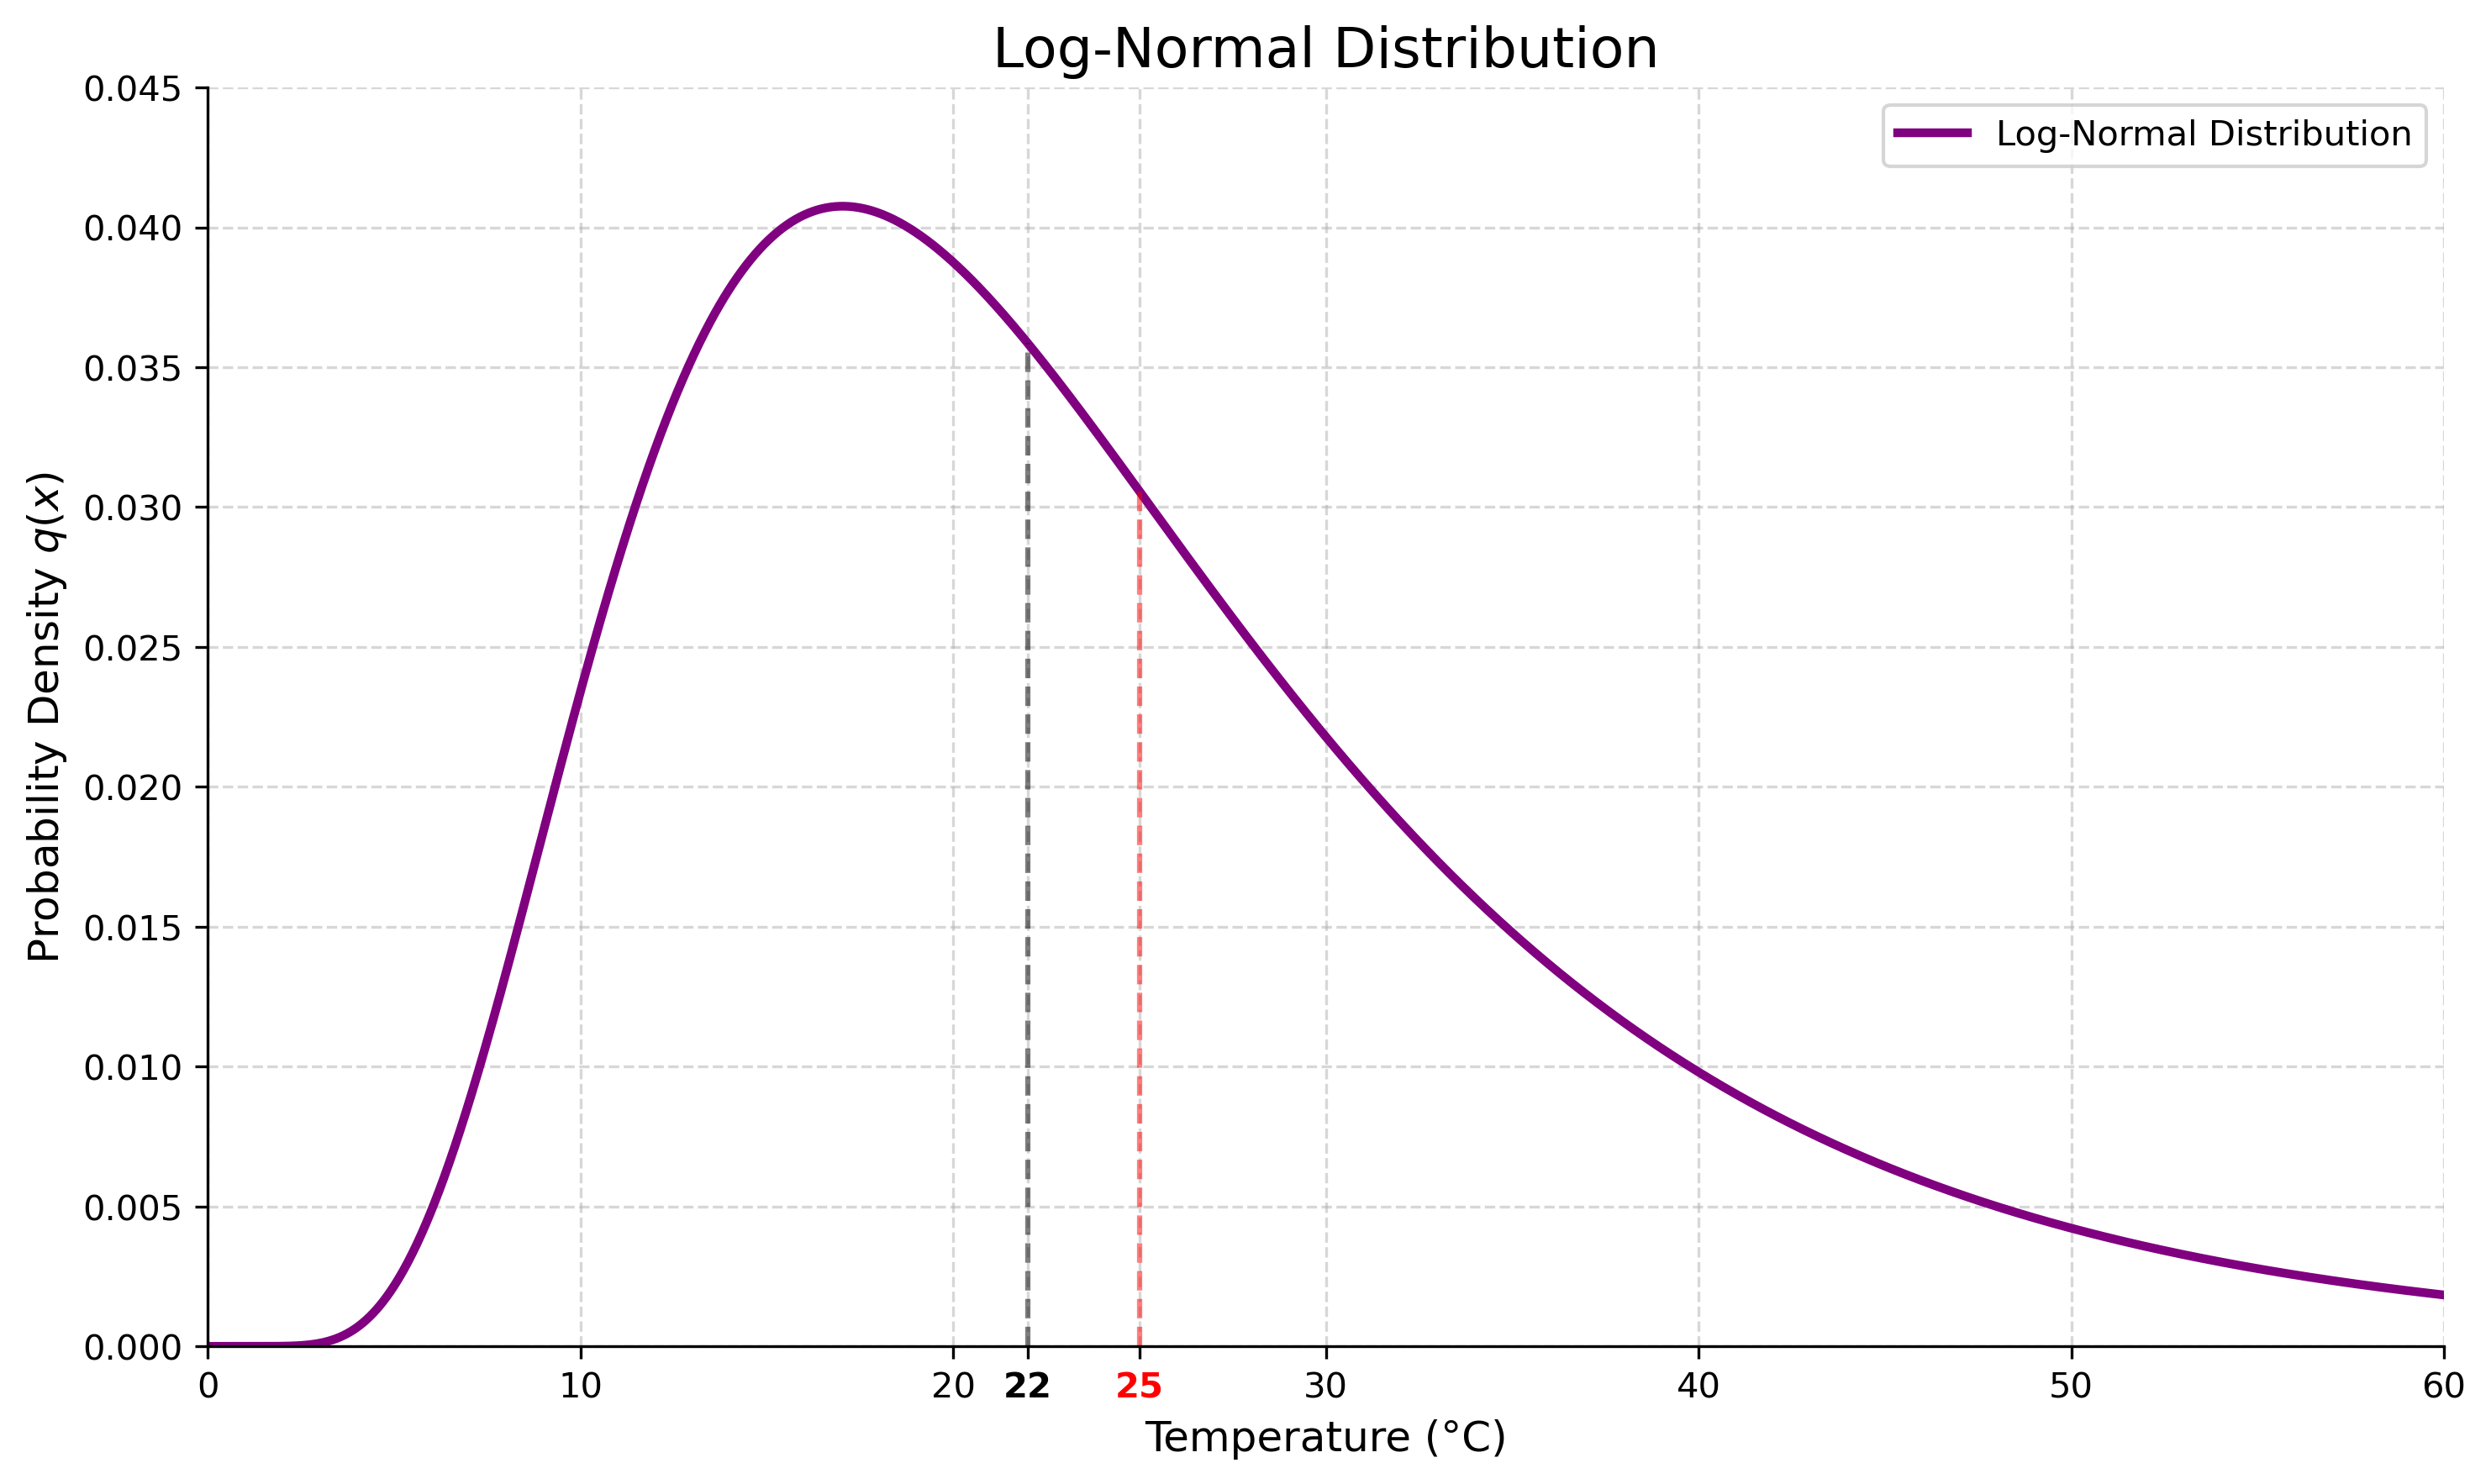
\includegraphics[width=0.6\linewidth]{images/lognormal_distribution.png}
    \end{figure}
\end{frame}




\section{Formulation}
\begin{frame}{Mathematical Characterization}
    \begin{block}{Definition}
        \begin{itemize}
            \item $\Omega$ sample space
            \item $\mathcal{A}$ $\sigma$-Algebra on subsets of $\Omega$
            \item $\mathcal{P}$ convex class of probability measures
            \item $P\in\mathcal{P}$ probabilistic forecast
        \end{itemize}
        \vspace{1em}
        $S:\mathcal{P}\times\Omega\to\overline{\mathbb{R}}: \, S(P, \cdot)$ quasi-integrable $\forall P\in\mathcal{P}$ is called a \textbf{Scoring Rule}. In the event $\omega$ the probabilistic forecast gives the \textbf{reward} $S(P,\omega)$.
    \end{block}
\end{frame}
\begin{frame}{Mathematical Characterization}
    \begin{block}{Definition}
        \begin{itemize}
            \item For $P, Q\in\mathcal{P}$ we define the \textbf{Expected Score}
            $$S(P,Q) = \mathbb{E}^{Q}\left[ S(P, \omega)\right] = \int_{\Omega} S(P, \omega)\mathrm{d}Q(\omega).$$
            \item $S$ is called \textbf{regular} relative to $\mathcal{P}$ if $$S(P, Q)\in[-\infty, \infty)\hspace{2em}$$ for all $P, Q \in\mathcal{P}$ where $P\neq Q$ and $S(P, P)\in \mathbb{R}$ for all $P\in\mathcal{P}$.
        \end{itemize}
    \end{block}
\end{frame}
\begin{frame}{Mathematical Characterization}
    \begin{block}{Definition}
        \begin{itemize}
            \item A scoring rule is called \textbf{proper} if $$S(Q, Q) \geq S(P, Q) \hspace{2em}\forall P,Q\in\mathcal{P}.$$
            \item A scoring rule is called \textbf{strictly proper} if $$S(Q, Q) > S(P, Q) \hspace{2em}\forall P,Q\in\mathcal{P},\ P\neq Q.$$
            \item Proper rules encourage honesty.
        \end{itemize}
    \end{block}
\end{frame}



\section{Divergences}
\begin{frame}{Divergences}
    \begin{block}{Definition}
        Let $S$ be proper relative to $\mathcal{P}$. The function $$G:\mathcal{P}\to\mathbb{R},\quad G(P) = \underset{Q\in\mathcal{P}}{\sup} S(Q, P)$$ is called the \textbf{information measure} or (generalized) \textbf{entropy function}.\\
    \end{block}
    Note: $G$ is \textit{convex} as $\sup$ over affine functions.
\end{frame}
\begin{frame}{Convexity}
    \begin{block}{Definition}
        A function $G:\mathcal{P}\to\mathbb{R}$ is \textbf{convex} if $$G\left( (1 - \lambda)P + \lambda Q \right) \leq (1 - \lambda) G(P) + \lambda G(Q)$$ for all $\lambda \in (0, 1)$ and $ P, Q \in \mathcal{P}$.
    \end{block}
\end{frame}
\begin{frame}{Divergence}
    \begin{block}{Definition}
        \begin{itemize}
            \item For a regular and proper scoring rule $S$ we call $$d:\mathcal{P}^2\to[0, \infty), \quad d(P, Q)= S(Q, Q) - S(P, Q)$$ the \textbf{divergence function}. 
            \item If $\Omega$ is finite, $G$ sufficiently smooth, then $d$ is the \textbf{Bregman divergence} associated with the (convex) entropy function $G$.
        \end{itemize}
    \end{block}
    Note: If $S$ is strictly proper, $d(P, Q)>0$ for $P\neq Q$.
\end{frame}
\begin{frame}{Bregman Divergence}
        \begin{figure}
            \centering
            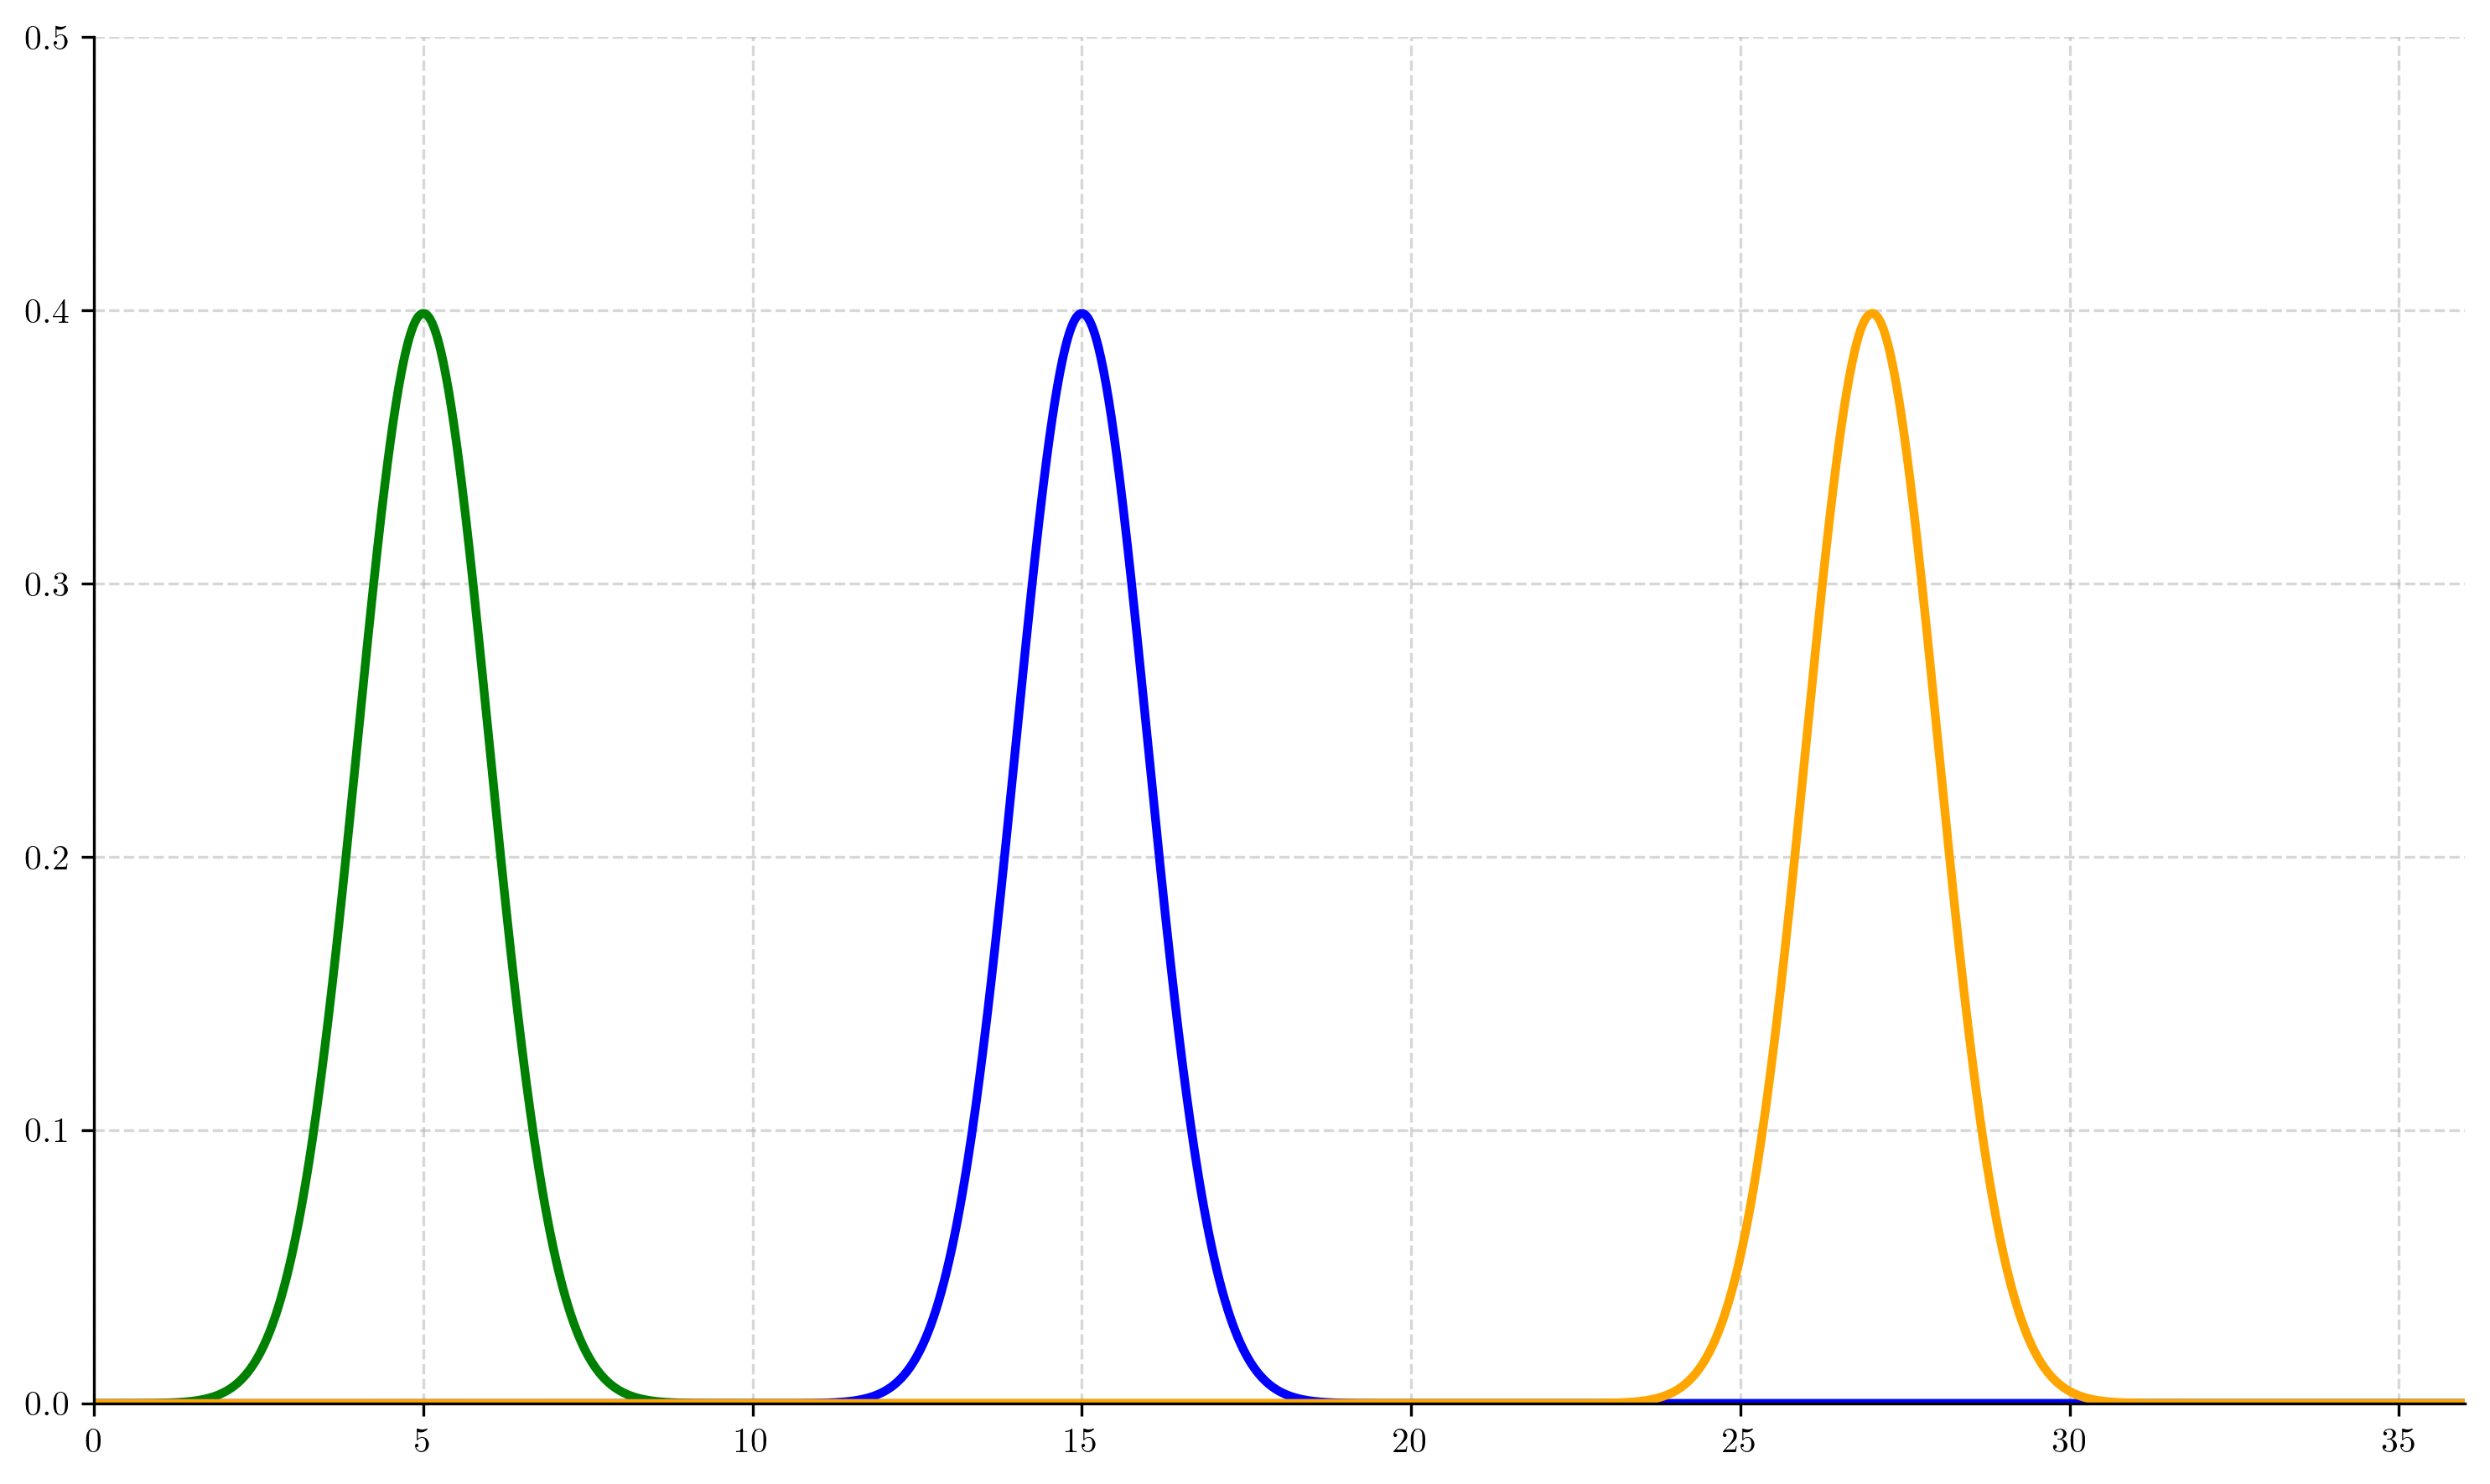
\includegraphics[width=\linewidth]{images/divergences.png}
        \end{figure}
\end{frame}




\section{Categorical SR}
\begin{frame}{Categorical Scoring Rules}
    \begin{block}{Setting}
        \begin{itemize}
            \item Let $\Omega = \{ 1, ..., n\}$ and $ \mathcal{P}=\Delta_n=\left\{ p\in\mathbb{R}^n:p\geq0, \sum_{j=1}^n p_j=1\right\}$. 
            \item $S(\cdot, i): \mathcal{P}\to\overline{\mathbb{R}}$.
        \end{itemize}
    \end{block}
    \begin{block}{Definition}
        Let $G:\mathcal{P}\to\mathbb{R}$ be convex. For $p\in\mathcal{P}$ the \textbf{subdifferential} of $G$ at $p$ is defined as $$\partial G(p) := \left\{ v\in\mathbb{R}^n: G(q)\geq  G(p) + \langle v, q-p\rangle \text{ for all } q\in\Delta_n \right \}.$$ A $v\in\partial G(p)$ is called a \textbf{subgradient}. Note: a subgradient is a vector in $\mathbb{R}^n$, not necessarily a probability vector.
    \end{block}
\end{frame}
\begin{frame}{Subdifferential}
    \begin{figure}
        \centering
        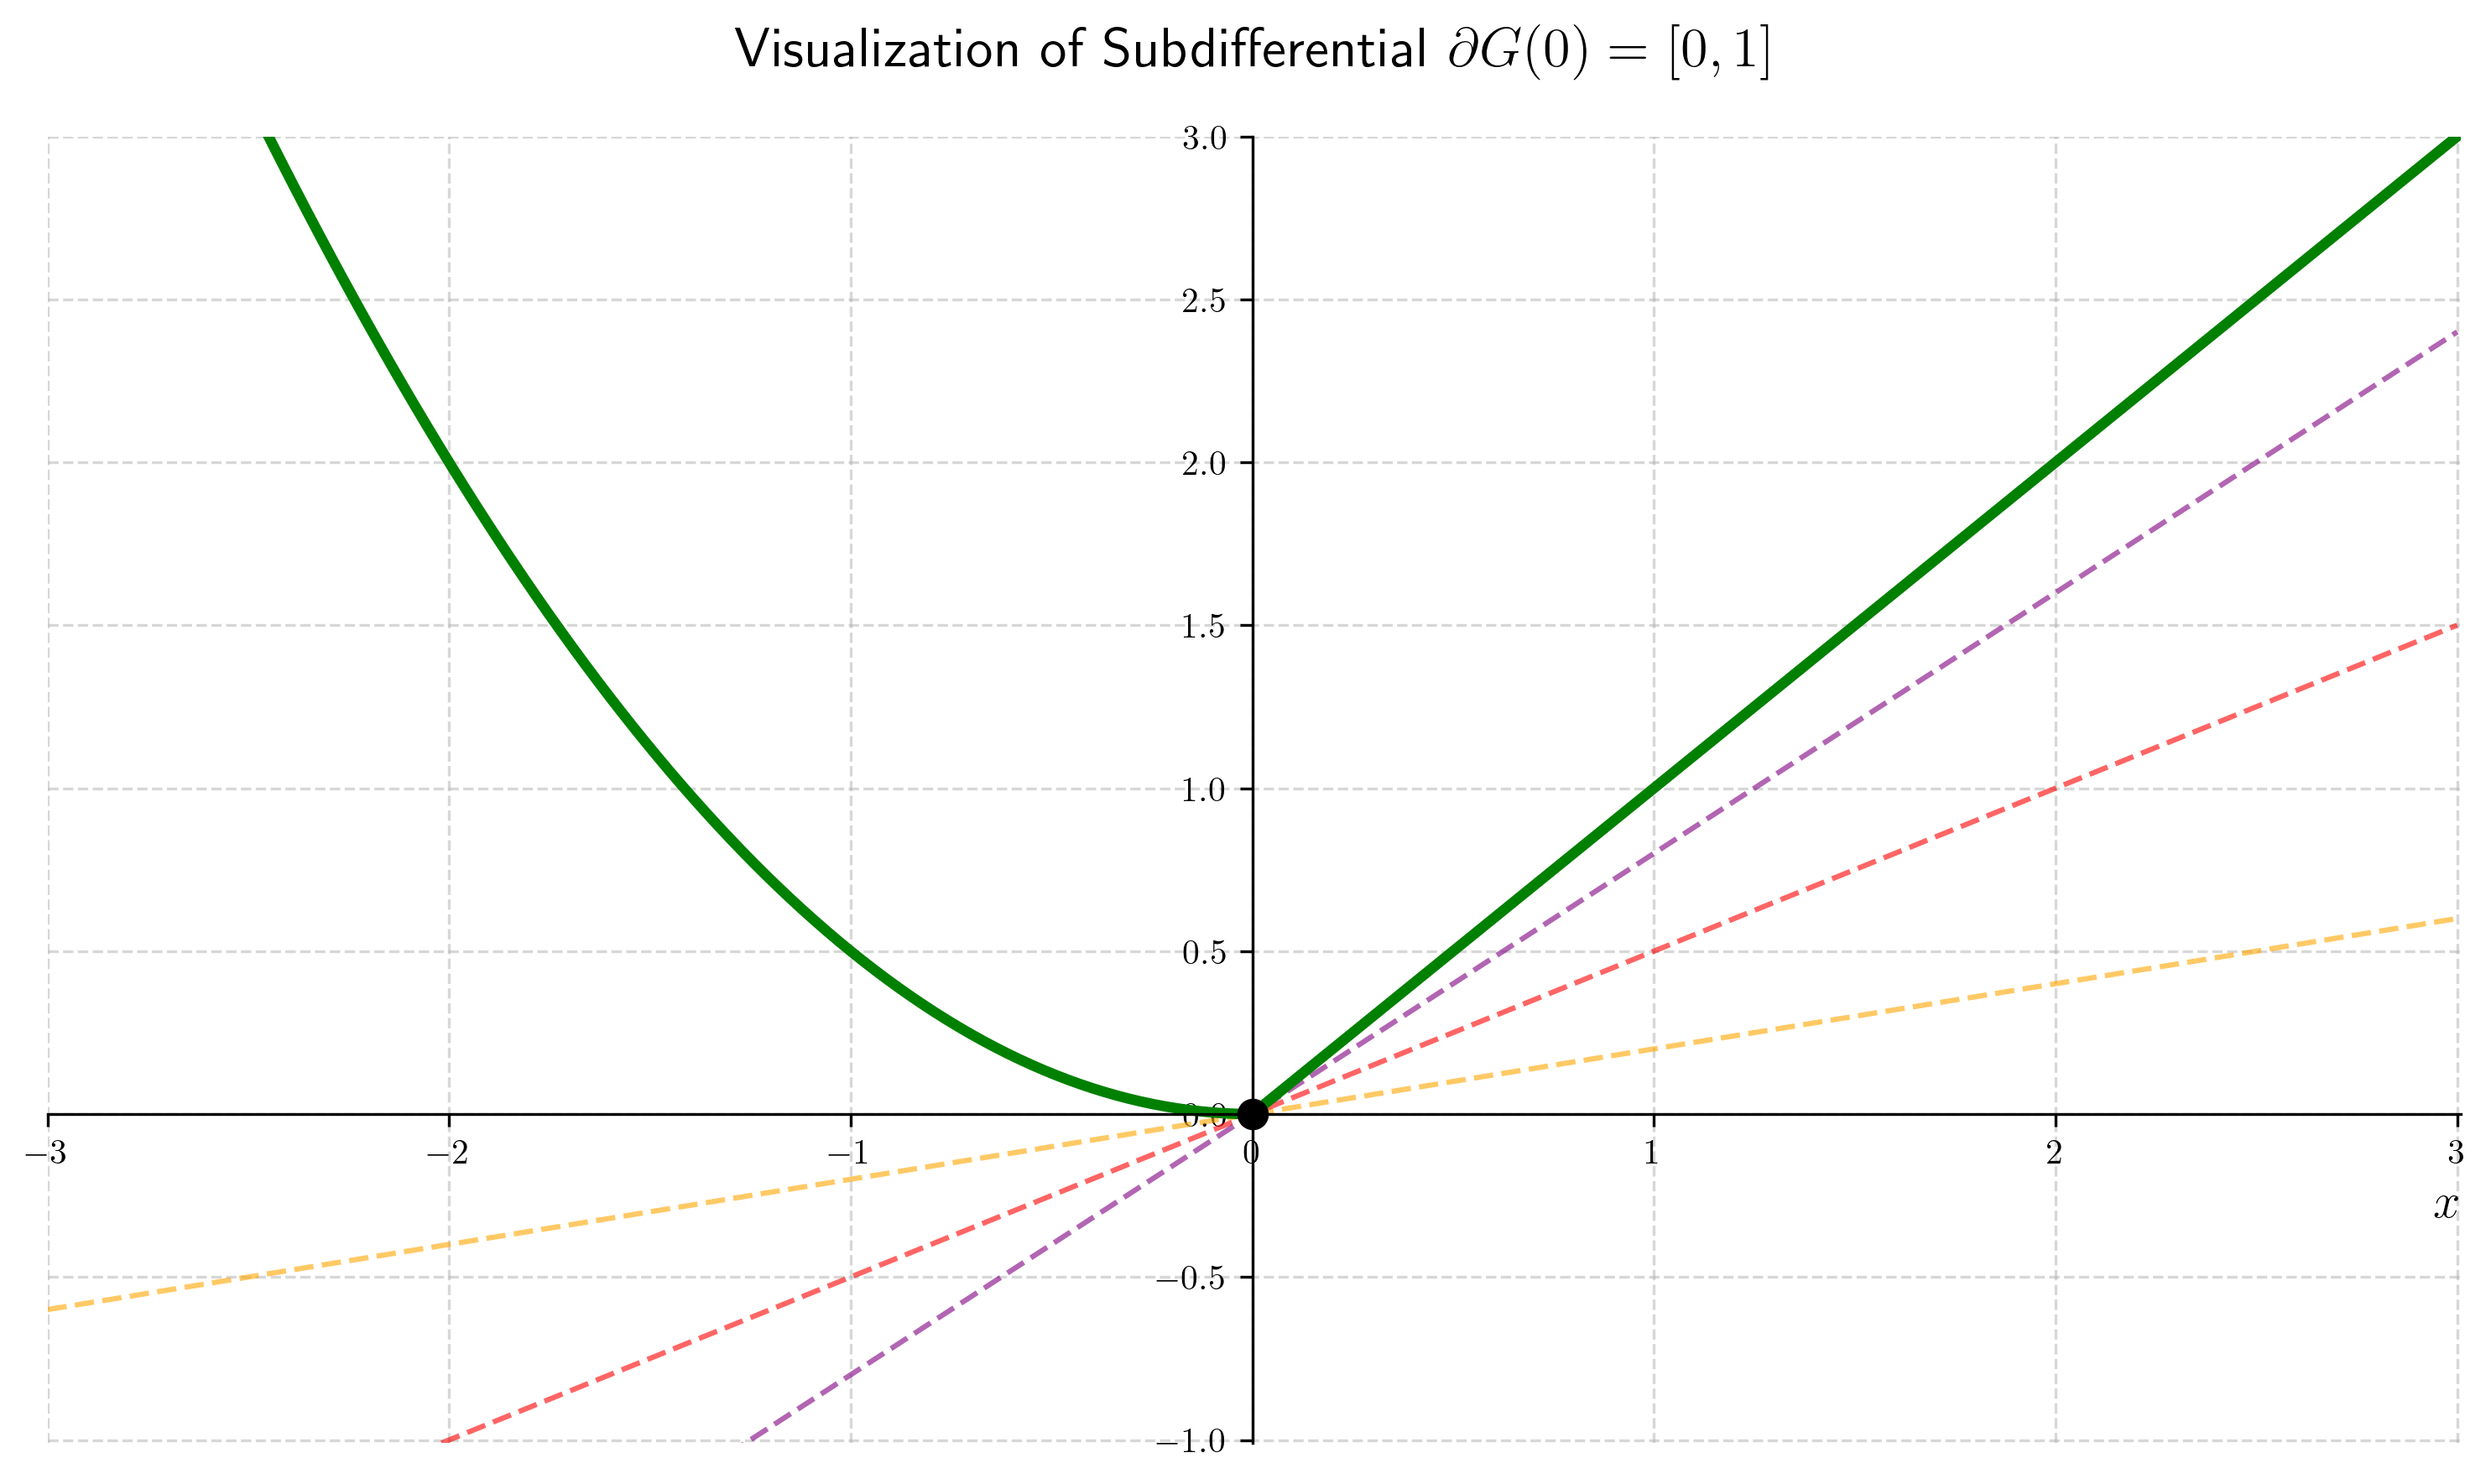
\includegraphics[width=\linewidth]{images/subgradient_visualization.png}
    \end{figure}
\end{frame}
\begin{frame}{Categorical Scoring Rules}
    \begin{block}{Theorem (McCarthy, Savage)}
        A scoring rule $S$ is proper if and only if $G(p)=S(p,p)$ is convex on $\mathcal{P}$ and $\sum_{i=1}^{n}S(p,i)e_i\in\partial G(p)$ for all $p\in\mathcal{P}$.
    \end{block}
    \begin{block}{Corollary}
        Every bounded convex entropy function $G$ on $\mathcal{P}$ generates a regular proper scoring rule.
    \end{block}
\end{frame}
\begin{frame}{Brier Score (Quadratic Score)}
    \begin{exampleblock}{Entropy Function}
        $$G(p) = \sum_{j=1}^n p_j^2-1$$
    \end{exampleblock}
    \begin{exampleblock}{Scoring Rule}
        $$S(p, i) = -\sum_{j=1}^n \left(\delta_{i,j} - p_j\right)^2 = 2p_i - \sum_{j=1}^np_j^2-1$$
    \end{exampleblock}
    \pause
    \begin{exampleblock}{Bregman Divergence}
        $$d(p, q) = \sum_{j=1}^n \left(p_j-q_j\right)^2$$
    \end{exampleblock}
\end{frame}
\begin{frame}{Logarithmic Score}
    \begin{exampleblock}{Entropy Function (Negative Shannon Entropy)}
        $$G(p) = \sum_{j=1}^n p_j\log(p_j)$$
    \end{exampleblock}
    \begin{exampleblock}{Scoring Rule}
        $$S(p, i) = \log(p_i)$$
    \end{exampleblock}
    \pause
    \begin{exampleblock}{Bregman Divergence (Kullback-Leibler Divergence)}
        $$d(p, q) = \sum_{j=1}^n q_j\log\left(\frac{q_j}{p_j}\right)$$
    \end{exampleblock}
\end{frame}
\begin{frame}{Zero-One Score}
    \begin{exampleblock}{Scoring Rule}
        $$S(p,i) = \begin{cases}
            1/\#M(p) & \text{if } i\in M(p) \\
            0 & \text{else}
        \end{cases}$$ where $$M(p) = \underset{1\leq j\leq n}{\arg\max}\ p_j$$ are the modes of $p$.
    \end{exampleblock}
    \begin{exampleblock}{Entropy Function}
        $$G(p) = \underset{1\leq j\leq n}{\max}\ p_j$$
    \end{exampleblock}
    \pause
    \begin{exampleblock}{Divergence Function}
        $$d(p, q) = \underset{1\leq j\leq n}{\max}\ q_j -\frac{\sum_{j\in M(p)}q_j}{\#M(p)}$$
    \end{exampleblock}
\end{frame}
\begin{frame}{Zero-One Score}
    Note: This is not a Bregman divergence, since $G$ is not differentiable and not strictly convex.
\end{frame}




























\section{SR for continuous variables}
%\subsection{subsection}

\begin{frame}
  \frametitle{Scoring Rules for Continuous Variables}
  Goal for this section:
  \begin{itemize}
    \item Define Scoring Rules for continuous variables
    \item See what the differences between them are
    \item Consider, what may be benefits or drawbacks of certain Scoring Rules
    \end{itemize}
\end{frame}

\subsection{Scoring of Density Forecasts}

\begin{frame}{Scoring Rules for Density Forecasts}
    Setting of the Forecasts:
    \begin{itemize}
        \item $\mu$ be $\sigma$-finite on $(\Omega,\mathcal A)$
        \item $\mathcal{L}_\alpha$ probability measures absolutely continuous with respect to $\mu$, $\alpha>1$
        \item Each measure from $\mathcal L_\alpha$ has $\mu$-density $p$ with \begin{equation*}
            \lVert p\rVert_\alpha=\left(\int p(\omega)^\alpha\mu(d\omega)\right)^{\frac 1\alpha}<\infty
        \end{equation*}
        \item $p$ will be called density forecast
    \end{itemize}
    Note: $p$ is not uniquely defined for some measure $P\in\mathcal L_\alpha$
\end{frame}
\subsection{Examples}
\begin{frame}{Examples for Scoring Rules for Density Forecasts}
\begin{itemize}
    \item Quadratic Score: \begin{equation*}
        \text{QS}(p,\omega)=2p(\omega)-\lVert p\rVert_2^2
    \end{equation*}
    \item Strictly proper relative to $\mathcal L_2$
    \item Expected score: \begin{equation*}
        G(p)=\lVert p\rVert_2^2
    \end{equation*}
\end{itemize}
    
\end{frame}

\begin{frame}{Examples for Scoring Rules for Density Forecasts}
    \begin{itemize}
        \item Pseudospherical Score: \begin{equation*}
            \text{PseudoS}(p,\omega)=\frac{p(\omega)^{\alpha-1}}{\lVert p\rVert_\alpha^{\alpha -1}}
        \end{equation*}
        \item Strictly proper relative to class $\mathcal L_\alpha$
    \end{itemize}
\end{frame}

\subsubsection{The logarithmic score}
\begin{frame}{The Logarithmic Score}
Definition: \begin{equation*}
    \text{LogS}(p,\omega)=\log p(\omega)
\end{equation*}
\begin{itemize}
    \item Strictly proper relative to $\mathcal L_1$ of dominated measures
    \item Widely used under various names
    \item Under certain conditions, all proper scoring rules that depend on $p$ only through the value $p(\omega)$ are equivalent
\end{itemize}
    
\end{frame}
%\section{other section}  
\begin{frame}{Using the Logarithmic Score (PASCAL Challenges)}
Setting (Regression task): \begin{itemize}
    \item Goal is to give a prediction for the correlation between variables
    \item Predictions given in form of density function
    \item Scoring of the prediction to determine a winner
\end{itemize}
\end{frame}
\begin{frame}{Scoring the Predictive Density}
    \begin{align*}
        L=\frac{1}{n}\sum_{i=1}^n\log p(y_i=t_i\mid x_i)
    \end{align*}
\end{frame}

\begin{frame}{Possible Problems of the Logarithmic Score}
    Expected point masses can dominate the score:\\
    \begin{figure}
    \centering
    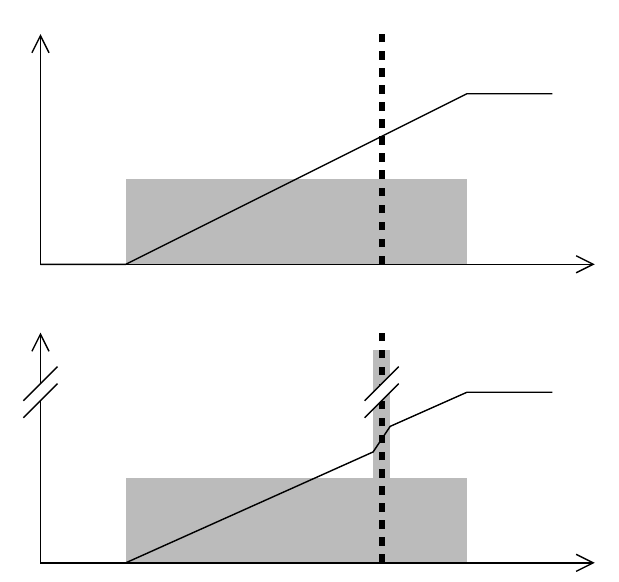
\includegraphics[width=0.5\textwidth]{images/Graphic Kohonen Suomela.png}
    \caption*{Fig. 1: Figure 8 of \cite{Kohonen} showing the issue with the logarithmic score}
    \end{figure}
\end{frame}

\begin{frame}{Possible Problems with this Scoring Function}
\begin{itemize}
    \item Setting artificially high densities could get rewarded
    \item Maybe looking at distributions functions could help
\end{itemize}
\end{frame}
\subsection{Scoring for cumulative distribution functions}
\begin{frame}{Scoring for Distribution Functions and CRPS}
    
\end{frame}

\begin{frame}{Scoring for Distribution Functions}
    Motivation for looking at distribution functions instead of densities:
    \begin{enumerate}
        \item Solving the point mass problem of logarithmic score
        \item Allowing samples to easily represent distribution functions:\begin{figure}
            \centering
            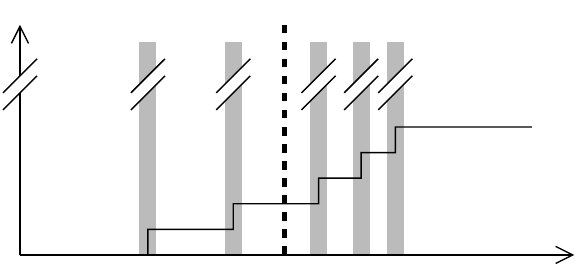
\includegraphics[width=0.5\linewidth]{images/Kohonen Suomela Fig.9.png}
            \caption*{Fig. 2: Figure 9 of \cite{Kohonen} about a way of representing a distribution function}
            \label{fig:placeholder1}
        \end{figure}
        \item Considering "distance"
    \end{enumerate}
\end{frame}

\subsection{CRPS}

\begin{frame}{Continuous Ranked Probability Score (CRPS)}
    \textbf{Definition:} $\mathcal P$ set of Borel probability measures on $\mathbb R$.\begin{equation*}
        \text{CRPS}(F,x)=-\int_{-\infty}^\infty (F(y)- \mathbbm{1} {\{y\geq x\}})^2 dy
    \end{equation*}
\end{frame}

\begin{frame}{Continuous Ranked Probability Score (CRPS)}

\begin{figure}
            \centering
            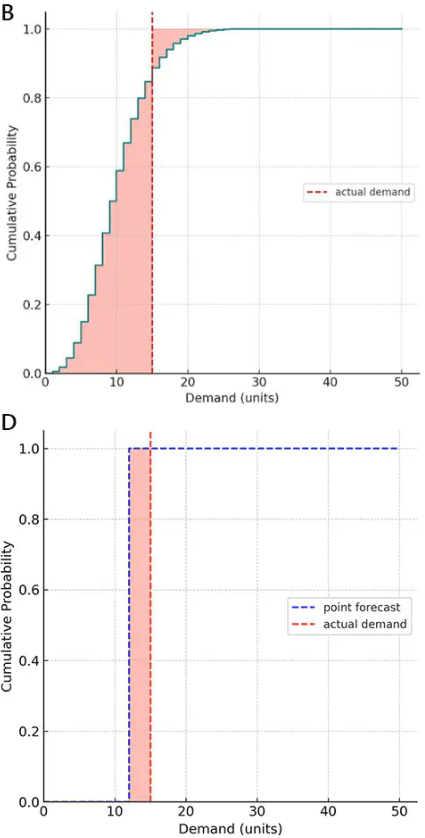
\includegraphics[width=0.25\linewidth]{images/lokad_CRPS.png}
            \caption*{Fig. 3: Visualisation of CRPS from https://www.lokad.com/continuous-ranked-probability-score/}
            \label{fig:CRPS-viz}
    \end{figure}
\end{frame}
\begin{frame}{Step by Step Visualisation}
\begin{figure}
    \centering
    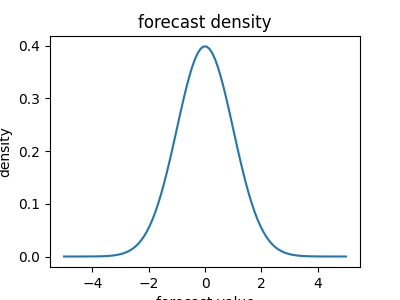
\includegraphics[width=0.33\linewidth]{images/Figure_1.png}
    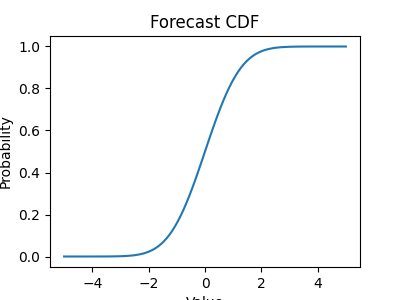
\includegraphics[width=0.33\linewidth]{images/Figure_4.png}
    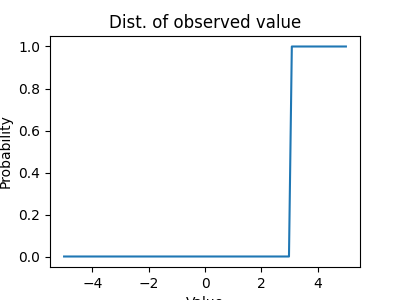
\includegraphics[width=0.33\linewidth]{images/Figure_2.png}
    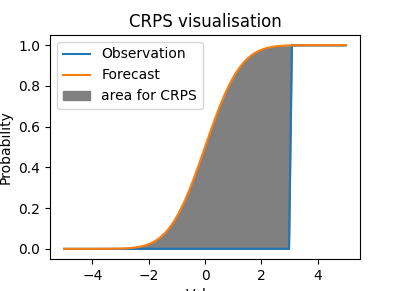
\includegraphics[width=0.33\linewidth]{images/Figure_3.png}
    \caption*{Fig. 4: Visualisation of the CRPS for predicted normal dist.}
    \label{fig:placeholder2}
\end{figure}
    
\end{frame}

\begin{frame}{Properties of the CRPS}
\begin{itemize}
    \item Proper relative to $\mathcal P$
    \item Strictly proper relative to subclass $\mathcal P_1$ of prob. measures with finite first moments
    \item Divergence function $$d(F,G)=\int_{-\infty}^\infty (F(y)-G(y))^2 dy$$
    \item Some sort of sensitivity for "distance"
\end{itemize}
    
\end{frame}

\begin{frame}{Properties of the CRPS}
\textbf{Alternative Definition:}\begin{equation*}
    \text{CRPS}(F,x)=\frac 12 E_F[\lvert X-X'\rvert]- E_F[\lvert X-x\rvert]
\end{equation*}
\begin{itemize}
    \item $X,X'$ independent copies of a random variable with dist. $F$
    \item Definition will come up again later
\end{itemize}
    
\end{frame}

\begin{frame}{Possible Downsides of the CRPS}
\begin{itemize}
    \item The integral is not always easy to compute
    \item One probably has to use numerical methods such as quadrature formulas: \begin{equation*}
        S=\sum_i (x_{i-1}-x_i)\cdot\frac{(F(x_{i-1})-D(x_{i-1})^2+(F(x_{i})-D(x_i))^2}{2}
    \end{equation*}
\end{itemize}
    
\end{frame}

\subsection{Other Scores to consider}
\begin{frame}{Possible other Scoring Functions}
\begin{itemize}
    \item Generalization of CRPS on $\mathbb R^m$ (energy score)
    \item Scoring rules only depending on first and second moment
\end{itemize}
\end{frame}
\section{Kernel Scores}
\begin{frame}{Kernel Scores}
    Is there a general way to describe or define Scoring Rules?
\end{frame}

\begin{frame}{Kernel Scores}
    \textbf{Definition (kernel)}: Let $\Omega$ be a nonempty set. A function $g\colon \Omega\times\Omega\to\mathbb R$ is called a negative definite kernel if it is symmetric in its arguments and \begin{equation*}
        \sum_{i=1}^n\sum_{j=1}^n a_ia_j g(x_i,x_j)\leq 0
    \end{equation*}
    for all positive integers $n$ and all $a_1,\dots,a_n$ that sum to $0$
\end{frame}

\begin{frame}{Kernel Scores}
\textbf{Theorem (Theorem 4 of \cite{Gneiting})}: Let $\Omega$ be a Hausdorff space (a space where distinct points have disjoint neighborhoods around them) and let $g\colon\Omega\times\Omega\to\mathbb R$ be a non-negative, continuous and negative definite kernel. Also let $P$ be a Borel probability measure on $\Omega$. Let $X,X'$ be independent with distribution $P$. In this case the scoring rule \begin{equation*}
    S(P,x)=\frac{1}{2}E_P[g(X,X')]-E_P[g(X,x)]
\end{equation*}
is proper regarding the class of Borel probability measures on $\Omega$
    
\end{frame}

\subsection{Examples}
\subsubsection{CRPS as kernel score}

\begin{frame}{CRPS as Kernel Score}
\begin{itemize}
    \item Take $g(x,x'):=\lvert x-x'\rvert$ as a kernel in our sense.
    \item The theorem then gives a score \begin{equation*}
        S(P,x)=\frac 12 E_P[\lvert X-X'\rvert]- E_P[\lvert X-x\rvert]
    \end{equation*}
\end{itemize}   
\end{frame}

\subsubsection{Brier Score as kernel Score}
\begin{frame}{Brier score}
    We look at the following scenario:
    \begin{itemize}
        \item $\Omega=\{0,1\}$
        \item $g(0,0)=g(1,1)=0$ and $g(1,0)=g(0,1)=1$
        \item $p_0,p_1$ as probabilities of each event $1$ or $0$
    \end{itemize}
    Then: \begin{equation*}
        S(P,1)=\frac{1}{2}(p_0p_1+p_1p_0)-p_0=p_0\cdot (1-p_0)-p_0=-p_0^2
    \end{equation*}
\end{frame}
\begin{frame}{Brier Score as Kernel Score}

\begin{figure}
            \centering
            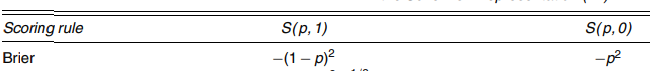
\includegraphics[width=1\linewidth]{images/Gneiting binary forecasts.png}
            \caption*{Fig. 5: Part of the Table in \cite{Gneiting} about Scores on binary forecasts} 
            \label{fig:placeholder3}
        \end{figure}

\end{frame}
\subsection{Further use of kernel scores}
\begin{frame}{Complex Kernel Scores}
We can allow complex-valued kernels $h$ as follows: \begin{itemize}
    \item $h\colon\Omega\times\Omega\to\mathbb C$ and $h(x,x')=\overline{h(x',x)}$
    \item $h$ positive definite: \begin{equation*}
        \sum_{i=1}^n\sum_{j=1}^n c_i\overline c_j h(x_i,x_j)\geq 0
    \end{equation*}
\end{itemize}
\end{frame}

\begin{frame}{Complex Kernel Scores}
    \textbf{General Idea:} Generalizing the theorem for this case. By doing that we can can look at $\mathbb R^m$ and choose $h$ the right way to get \begin{equation*}
        S(P,x)=-\lvert \phi_P(y)-e^{i\langle x,y\rangle}\rvert^2.
    \end{equation*}
    Here $\phi_P$ is the characteristic function of the predictive distribution.
\end{frame}

\section{SR for quantiles}
\begin{frame}{Scoring Rules for Quantiles}
\begin{itemize}
    \item Instead of predictive distributions we look at sections of the distribution
    \item The predictions now are the points at the edges of these sections
\end{itemize}
    
\end{frame}

\begin{frame}{Motivation for Quantile Scores (Value at Risk)}
\begin{figure}
    \centering
    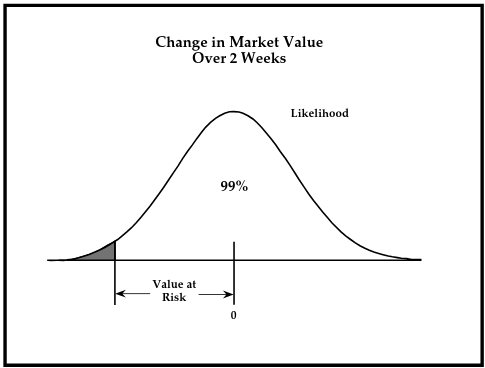
\includegraphics[width=0.75\linewidth]{images/VaR.png}
    \caption*{Fig. 6:Figure 1 of \cite{VaR} for a intuition behind the VaR}
    \label{fig:placeholder4}
\end{figure}
    
\end{frame}

\begin{frame}{Intuition behind Quantiles}
\textbf{Setting:} We want to have the values $r_1,\dots,r_k$ at given probability levels $\alpha_1,\dots,\alpha_k\in (0,1)$ such that \begin{equation*}
    P(x\leq r_k)=\alpha_k.
\end{equation*}
We are trying to score the predicted values $r_k$.
\end{frame}

\begin{frame}{Proper Scoring Rules for Quantiles}
\begin{itemize}
    \item Let $q_1,\dots,q_k$ denote the true quantiles of distribution $P$
    \item Scoring rules for quantiles will have the form $S(r_1,\dots,r_k,x)$ with \begin{equation*}
        S(r_1,\dots,r_k,P)=\int S(r_1,\dots,r_k,x)dP(x).
    \end{equation*}
    \item A Scoring Rule is called proper if \begin{equation*}
        S(q_1,\dots,q_k,P)\geq S(r_1,\dots,r_k,P)
    \end{equation*}
    for all $r_1,\dots,r_k\in\mathbb R$ and probability measures $P$.
\end{itemize}
\end{frame}
\begin{frame}{Proper Scoring Rules for Quantiles}
\textbf{Theorem:} Let $s$ be a nondecreasing function and $h$ an arbitrary function, then \begin{equation*}
    S(r,x)=\alpha s(r)+(s(x)-s(r))\mathbbm 1_{\{x\leq r\}} +h(x)
\end{equation*}
is proper for predicting a single quantile at level $\alpha\in (0,1)$.
    
\end{frame}

\begin{frame}{Scoring Multiple Quantiles}
\begin{itemize}
    \item Choose $s_i, i=1,\dots,k$ as in the theorem and
    \item $h$ arbitrary
    \item The sum over all scores $i=1,\dots,k$ is proper for scoring $k$ quantiles
\end{itemize}
\end{frame}
\begin{frame}{Example}
    Set $s(x)=x, h(x)=-\alpha x$. Then we get the Score \begin{equation*}
        S(r,x)=\alpha r+(x-r)\mathbbm 1_{\{x\leq r\}}-\alpha x=(x-r)(\mathbbm 1_{\{x\leq r\}}-\alpha)
    \end{equation*}
\end{frame}
\begin{frame}{Special Case: Interval Score}
    \begin{itemize}
        \item Prediction of quantiles at $\frac{\alpha}{2}, 1-\frac\alpha 2$
        \item E.g. prediction of central 50\% by using $\alpha=\frac12$
        \item Can be scored like quantiles
    \end{itemize}
\end{frame}
\section{Comparison}
\begin{frame}{Potential Further Applications}
    \begin{itemize}
        \item Use Scoring Rules to score forecasting models
        \item Let $X=(X_1,\dots,X_n)$ 
        \item Forecast of a model determined up to a parameter $\theta$
    \end{itemize}
\end{frame}
\begin{frame}{Scoring Function in this Applications}
Comparing Forecasting Models:
\begin{itemize}
    \item Basic score: \begin{equation*}
        S_{k,B}=\sum_{t=1}^n \log p(X_t\mid X^{t-1},H_k)
    \end{equation*}
\end{itemize}
    
\end{frame}
\begin{frame}{Unordered Data}
If the observed data does not arrive in a certain order we look at random samples with random uniformly distributed size. The modification of the score from before opens up the possibility of cross-validation
    
\end{frame}












\appendix
\newcounter{finalframe}
\setcounter{finalframe}{\value{framenumber}}
\nocite{Gneiting}
\nocite{Unger}
\nocite{Candela}
\begin{frame}[noframenumbering]{References}
\bibliographystyle{plain}
\bibliography{References/refs}
\end{frame}

\begin{frame}{Further References}
    CRPS-Visualization code: {https://scores.readthedocs.io/en/stable/tutorials/CRPS\textunderscore for\textunderscore CDFs.html}\\
    
    Figure 3: https://www.lokad.com/continuous-ranked-probability-score/
    
\end{frame}
\end{document}
